\documentclass{report}
\usepackage{graphicx} % Required for \includegraphics
\usepackage{float}    % Required for [H] specifier

\begin{document}
\title{Labwork 5: Report}
\author{Nguyen Nhat Anh} % Required by the report class for \maketitle
\maketitle

\section{Introduction}
I have made the image Gaussian Blur Convolution using Numba CUDA. All the code given are following strictly from report. 

\section{Results}
For CPU:
\begin{figure}[H]
    \centering 
    \includegraphics[width=0.7\linewidth]{output_cpu.jpg}
    \caption{CPU image blur output.}
    \label{fig:cpu_image} 
\end{figure}

For GPU:
\begin{figure}[H]
    \centering 
    \includegraphics[width=0.7\linewidth]{output_basic.jpg}
    \caption{GPU image without shared memory blur output.}
    \label{fig:gpu_image_no_shared}
\end{figure}

\begin{figure}[H]
    \centering 
    \includegraphics[width=0.7\linewidth]{output_shared.jpg}
    \caption{GPU image with shared memory blur output.}
    \label{fig:gpu_image_shared}
\end{figure}

Performance comparison:
\begin{figure}[H]
    \centering 
    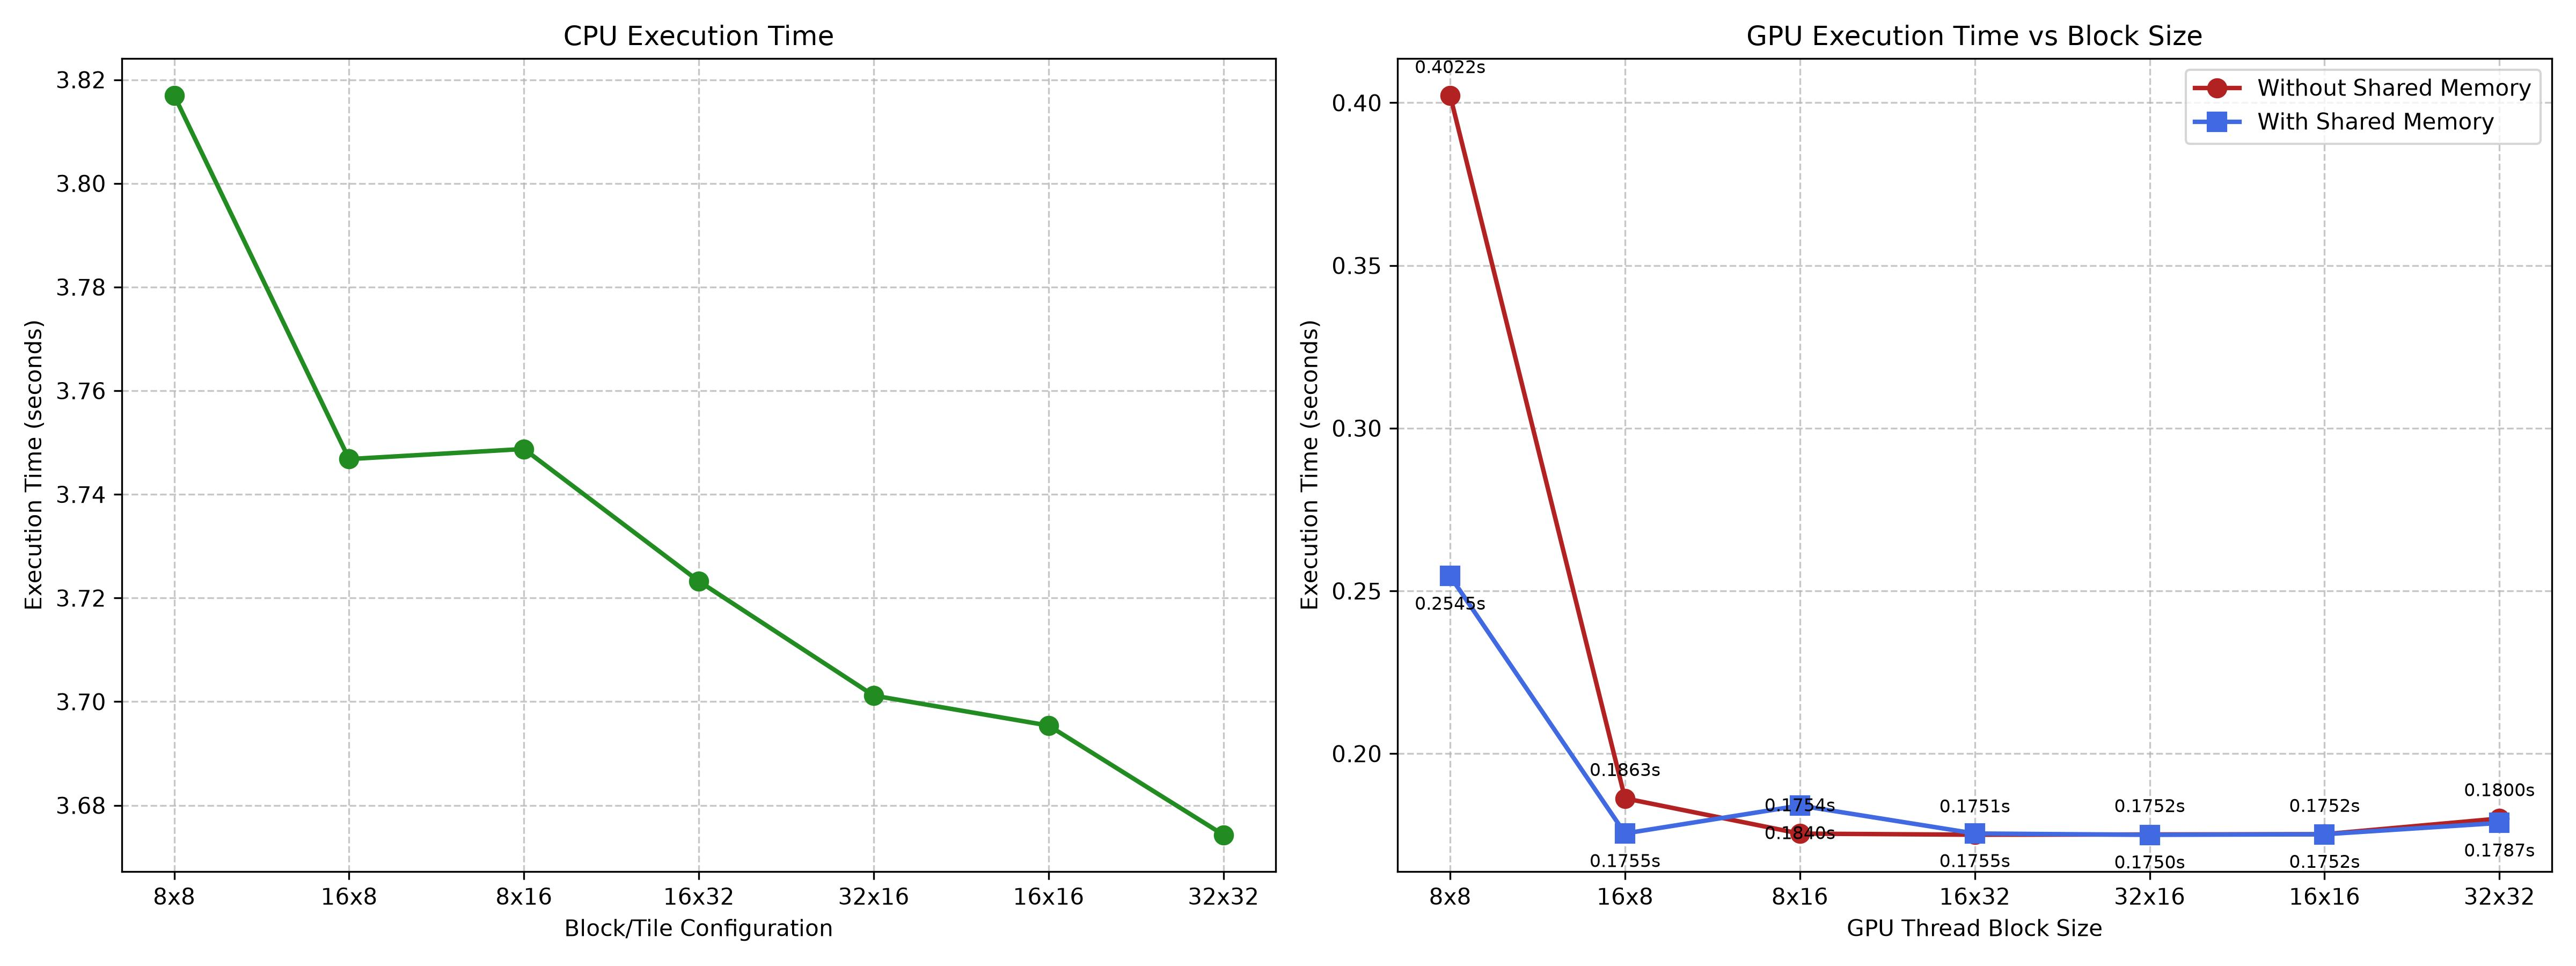
\includegraphics[width=0.7\linewidth]{blur_performance.jpg}
    \caption{Performance comparison.}
    \label{fig:performance_image}
\end{figure}
\section{Discussion}
In GPU experiment, the shared memory shows the improvements for the 8x8 block size,
for the other NxN block sizes show the same performance for the non-shared memory. 
In 16x8, the shared memory is better optimization than the non-shared memory and vice-versa for 8x16.
\end{document}